\documentclass{scrartcl}

\usepackage{graphicx} % Required for the inclusion of images

\renewcommand{\labelenumi}{\alph{enumi}.}
% deutsche Sprache und Umlaute
\usepackage[utf8x]{inputenc}
\usepackage[ngerman]{babel}


%BibTex verweise
\usepackage{cite}

% für url pfade
\usepackage{url}

% setzt beim neuen Absatz das erste Wort 4 mm nach rechts \\ kleine Abstand vom Rand
\setlength{\parindent}{4mm}

%für boxen
\usepackage{pifont,mdframed}

\usepackage{microtype}

% hack für scr paket für Indexierung
\usepackage{scrhack}

% erzwingen der Positionierung
\usepackage{float}
\restylefloat{figure}

% Verbindungen vom Index, Tabellen und Abbildungen
\usepackage{hyperref}

%Tiefe des Inhaltsverzeichnis
\setcounter{tocdepth}{5}

%für Unterstriche
\usepackage{underscore}

% Beschriftung
\usepackage{caption}
\captionsetup{%
  font=small,
  labelfont=bf,
}

\usepackage{fancybox}

%\geometry{showframe}% for debugging purposes -- displays the margins

\usepackage{amsmath}
\usepackage{amssymb}
\usepackage{geometry}
\geometry{verbose,a4paper,tmargin=20mm,bmargin=25mm,lmargin=15mm,rmargin=20mm}
% Set up the images/graphics package

% The following package makes prettier tables.  We're all about the bling!
\usepackage{booktabs}

% The units package provides nice, non-stacked fractions and better spacing
% for units.
\usepackage{units}

% The fancyvrb package lets us customize the formatting of verbatim
% environments.  We use a slightly smaller font.
\usepackage{fancyvrb}
\fvset{fontsize=\normalsize}

% Small sections of multiple columns
\usepackage{multicol}

% Provides paragraphs of dummy text
\usepackage{lipsum}

% listing
\usepackage{listings}
\usepackage{color}
\definecolor{grey}{rgb}{0.4,0.4,0.4}
\definecolor{darkblue}{rgb}{0.0,0.0,0.6}
\definecolor{cyan}{rgb}{0.0,0.6,0.6}

\lstset{
  basicstyle=\tiny,
  columns=fullflexible,
  showstringspaces=false,
  commentstyle=\color{gray}\upshape
}

\lstdefinelanguage{XML} {
  morestring=[b]",
  morestring=[s]{>}{<},
  morecomment=[s]{<?}{?>},
  stringstyle=\color{black},
  identifierstyle=\color{darkblue},
  keywordstyle=\color{cyan},
  morekeywords={xmlns,version,type}
}

\makeatletter
\newenvironment{CenteredBox}{%
\begin{Sbox}}{% Save the content in a box
\end{Sbox}\centerline{\parbox{\wd\@Sbox}{\TheSbox}}}% And output it centered
\makeatother



\title{Rechnersicherheit - Übung 04}
\author{Dennis Hägler und Martin Görick \\ Tutor: Stefan Pfeiffer}
%\date{\today}  % if the \date{} command is left out, the current date will be used


\begin{document}
\maketitle


\section*{Aufgabe 1}
Zuerst wird mittels einer Blockchiffre aus dem geheimen Schlüssel $K$ zwei Schlüssel $K_1$ und $K_2$ generiert.
Danach wird die MAC nach Abbildung \ref{fig:cmac} generiert.

\textbf{CHIP} ist die Blockchiffre mit dem geheimen Schlüssel K
\textbf{$MBS_{Tlen}$} ist die Länge der MAC

\begin{figure}[thp]
  \begin{CenteredBox}
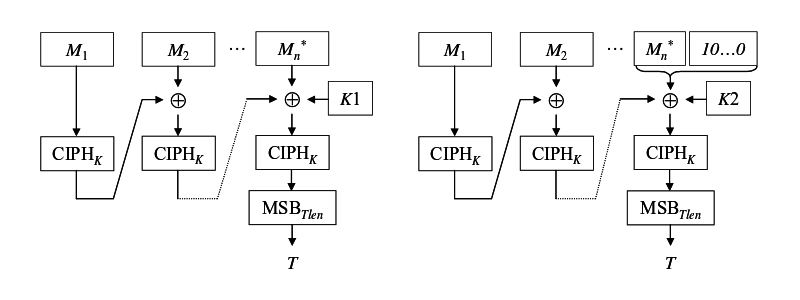
\includegraphics[scale=0.5]{CMAC}
  \end{CenteredBox}
  \caption{MAC generierung}
  \label{fig:cmac}
\end{figure}

Zur Verifikation wird aus dem $K,M$ ein $T'$ berechnet und mit dem übermittelten $T$ verglichen.

\paragraph*{Quelle}
Recommendation for Block Cipher Modes of Operation: The CMAC Mode for Authentication, Morris Dworkin, 	NIST Special Publication 800-38B, May 2005.


\section*{Aufgabe 2}
\begin{itemize}
\item[1] Ein Empfänger welcher den Schlüssel zum vergleichen hat, könnte mit
  einer zufälligen Signatur, zufällige aussehende Texte erstellen. Damit kann
  verhindert werden, dass der Sender zufällige Texte wie Schlüssel signieren
  kann, da nicht sicher ist ob die zufälligen Texte vom Sender sind.
\item[2] Ein Empfänger will aus einem Text m und einer Signatur s ein eigenes Dokument $m''$ mit der gültigen Signatur $s''$ erzeugen. Unter einem Vorwand soll der Sender ein Dokument $m' = m^{-1} * m''$ signieren. Der Sender soll keinen Verdacht schöpfen, da $m'$ unsinnig ist. Mit der erhaltenen Signatur $s'$ unter mod n gerechnet und mit dem privaten Schlüssel $d$ erhält der Angreifer ein $s''$ wie folgt.
$$s'' = s * s' = m^d * m'^d = (m*m')^d = (m*m6{-1} * m'')^d = m''^d$$
\end{itemize}

\paragraph*{Quelle}
RSA-Signatur,Hans Werner Lang, 2014, \url{http://www.iti.fh-flensburg.de/lang/krypto/protokolle/rsa-signatur.htm}

\section*{Aufgabe 3}

\begin{itemize}
\item[a)] In der Menge $\mathbb{Z}^*_p (g)$ sind alle Möglichkeiten enthalten, den geheimen Schlüssel zu wählen. Dieser wird aus 4. $a$ gewählt wie beschrieben geht a von 1 bis $q-1$. Theoretisch könnte jedoch auch q als geheimer Schlüssel gewählt werden. Diese Zahl ist jedoch bekannt, weshalb diese nicht verwendet wird. Also sind in der Menge $\mathbb{Z}^*_p (g)$ genau q Elemente mit allen möglichen Elementen von $A$ sowie $g^q$.
\item[b)] q muss mindestens eine Länge von 224 Bit und p 2048 Bit Länge besitzen.
\end{itemize}

\section*{Aufgabe 4}
\begin{itemize}
\item $G$ ist ein fester Erzeuger der n-Torsionsuntergruppe der Kurve
\item $n$ ist die Ordnung des Punktes G
\item $L_n$ die Bitlänge der Gruppenordnung n
\end{itemize}

\subsection*{Schlüsselerzeugung}
\begin{itemize}
\item privat key (sk) ist ein zufällige Ganzzahl zwischen $1$ und $n-1$
\item public key $pk = sk * G$
\end{itemize}

\subsection*{Signaturerzeugung}
Signatur für Nachricht m erzeugen mit Hashfunktion H.
\begin{itemize}
\item[1.] berechne $e = H(m)$ und definiere $z$ mit den $L_n$ hochwertigsten Bits von $e$  
\item[2.] wähle zufällige Ganzzahl $k$ von 1 bis n-1
\item[3.] berechne $r = x_1 (\text{mod } n) $, wobei $(x_1, y_1) = k * G$, wenn $r = 0$ gehe zu 2.
\item[4.] berechne $s = k^{-1} ( z + r * sk) (\text{mod } n)$($z$ wird in eine Ganzzahl umgewandelt), wenn $s = 0$ gehe zu 2.
\item[5.] Signatur ist das Paar $(r,s)$
\end{itemize}

\subsection*{Überprüfen der Signatur}
Wenn nicht sicher ist ob der pk richtig erzeugt wurde muss dieser überprüft werden.
\begin{itemize}
\item Überprüfen ob pk nicht das neutrale Element der Kurve ist und es valide Koordinaten.
\item Überprüfen ob pk auf der Kurve liegt.
\item überprüfe ob n*pk = neutrales Element, es wird überprüft ob pk ein Vielfaches von G ist.
\end{itemize}

Signatur überprüfen in den Folgenden Schritten:
\begin{itemize}
\item überprüfen ob r und s ganze Zahlen und im Intervall von $1$ bis $n-1$, wenn nicht Signatur ungültig
\item berechne $e = H(m)$ und definiere $z$ mit den $L_n$ hochwertigsten Bits von $e$
\item berechne $w = s^{-1} (\text{mod } n)$
\item berechne $u_1 = z * w 	(\text{mod } n)$ und $u_2 = r * w (\text{mod } n)$
\item berechne $(x_1,y_1) = u_1 G + u_2 pk$
\item Signatur ist gültig, wenn $r = x_1 (\text{mod } n)$ 
\end{itemize}

\paragraph*{Quelle}
Wikipedia \url{http://de.wikipedia.org/wiki/Elliptic_Curve_DSA}
\end{document}

